\section{Resultados da RQ 07}

A RQ 07 compara a classificação geral dos repositórios nas combinações C1, C2 e C3 (Seção~\ref{sec:definicoes}), repositório a repositório, pelo percentual que muda de categoria e pelo kappa de Cohen ponderado linear. Ficam fora do par os repositórios com C2 ou C3 indefinida: \texttt{zed-industries/zed} (sem lead time (b) e CFR (b) em C2) e \texttt{docling-project/docling} (sem as tags de C3), porque a API devolveu HTTP 422 em uma consulta de cada um. Por isso os pares têm 299, 299 e 298 repositórios.

\begin{table}[ht]
\centering
\small
\caption{Concordância entre as classificações gerais de cada par de combinações (Mudam = repositórios que trocam de categoria; Vizinha = trocas de uma só categoria; Sobem e Descem = sentido da troca de $x$ para $y$).}
\label{tab:rq07_pares}
\begin{tabular}{lrrrrrrl}
\hline
Par ($x \times y$) & n & Mudam & \% & Vizinha & Sobem & Descem & $\kappa$ \\
\hline
C1 $\times$ C2 & 299 & 90 & 30,1 & 83 & 26 & 64 & 0,544 (moderada) \\
C1 $\times$ C3 & 299 & 65 & 21,7 & 61 & 49 & 16 & 0,685 (substancial) \\
C2 $\times$ C3 & 298 & 85 & 28,5 & 82 & 81 & 4 & 0,591 (moderada) \\
\hline
\end{tabular}
\end{table}

Entre 21,7\% e 30,1\% dos repositórios mudam de categoria conforme a definição (Tabela~\ref{tab:rq07_pares}), 92\% a 97\% delas para uma categoria vizinha, e nenhum vai de \textit{Elite} para \textit{Low}, ou o contrário. A Figura~\ref{fig:rq07} mostra que, em C1$\times$C2, só 6 dos 24 repositórios \textit{Elite} de C1 continuam \textit{Elite} (13 passam a \textit{High} e 5 a \textit{Medium}), enquanto em C1$\times$C3 17 dos 24 continuam.

\begin{figure}[ht]
\centering
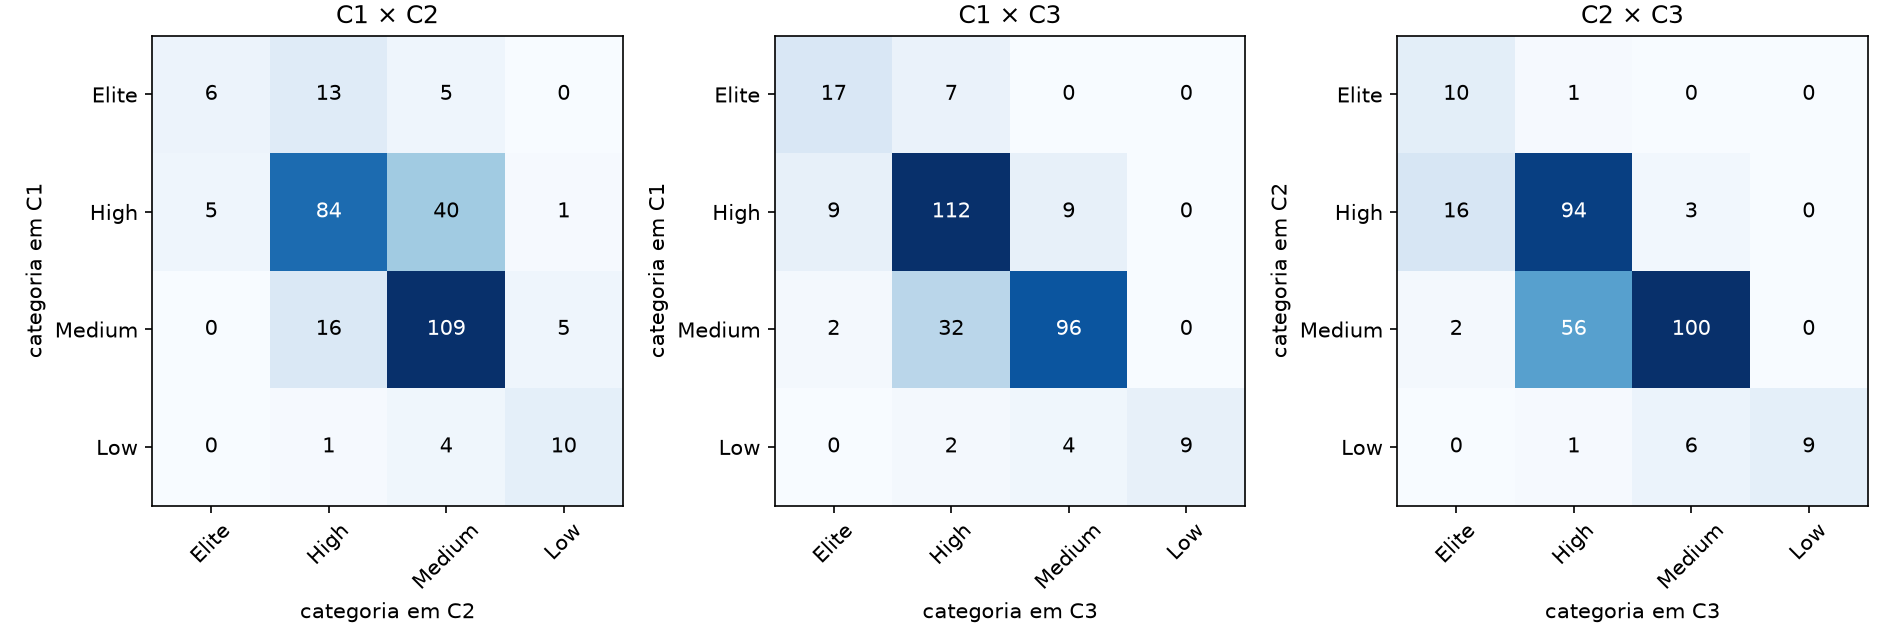
\includegraphics[width=0.88\textwidth]{rq07_matrizes.png}
\caption{Matrizes de transição entre as categorias gerais de cada par de combinações (as linhas são a categoria na primeira combinação, e as colunas, na segunda).}
\label{fig:rq07}
\end{figure}

A distribuição agregada também muda: os \textit{Elite} são 24 em C1, 11 em C2 e 28 em C3, e a categoria mais comum é a \textit{High} em C1 (por um repositório) e em C3 (51,2\%), mas a \textit{Medium} em C2 (52,8\%).

\begin{table}[ht]
\centering
\small
\caption{Mudança de faixa de cada métrica entre as combinações: \% de repositórios cuja nota muda e, entre parênteses, quantos sobem e quantos descem de $x$ para $y$. O CFR de C1 e C3 é o mesmo (CFR (a)).}
\label{tab:rq07_metricas}
\begin{tabular}{lrrr}
\hline
 & C1 $\times$ C2 & C1 $\times$ C3 & C2 $\times$ C3 \\
\hline
Frequência de deploy & 10,7 (32/0) & 25,1 (75/0) & 15,1 (45/0) \\
Lead time & 43,6 (66/64) & 46,6 (75/64) & 10,1 (21/9) \\
CFR & 59,3 (29/147) & 0,0 (0/0) & 59,3 (147/29) \\
Classificação geral & 30,1 (26/64) & 21,7 (49/16) & 28,5 (81/4) \\
\hline
\end{tabular}
\end{table}

A Tabela~\ref{tab:rq07_metricas} mostra de onde vêm as trocas. O CFR muda de faixa em 59,3\% dos repositórios entre C2 e as demais, quase sempre para pior em C2, cujo CFR (b) tem mediana de 17,0\%, contra 4,7\% do (a). O lead time muda em 43,6\% a 46,6\% entre C1 e as demais, nos dois sentidos (medianas de 255,7 h em C1, 264,1 h em C2 e 215,6 h em C3), mas em só 10,1\% entre C2 e C3, que usam a mesma variante. A frequência só sobe: a mediana passa de 0,54 para 0,65 (C2) e 0,88 (C3) por semana. Como a categoria geral é a mediana de quatro notas, parte das trocas é absorvida.

\begin{table}[t]
\centering
\small
\caption{Hipóteses da RQ 07 frente aos resultados.}
\label{tab:hipoteses_rq07}
\begin{tabular}{p{0.55\textwidth}p{0.37\textwidth}}
\hline
Hipótese & Resultado \\
\hline
20\% a 40\% mudam de categoria em cada par & Confirmada (21,7\% a 30,1\%) \\
Mudanças quase sempre para uma categoria vizinha & Confirmada (92\% a 97\%) \\
Kappa ponderado moderado a substancial & Confirmada (0,544 a 0,685) \\
C2 e C3 levam a categorias melhores que C1 & Confirmada só para C3 \\
Pré-releases e tags aumentam a frequência & Confirmada \\
Lead time (b) menor que o (a) & Parcial: só em C3 \\
Maior divergência em C1$\times$C2, menor em C2$\times$C3 & Parcial: a menor é C1$\times$C3 \\
Variação por métrica maior que a da geral & Parcial: não na frequência \\
\hline
\end{tabular}
\end{table}

\subsection{Discussão}

A escolha da definição não inverte o desempenho de um repositório, mas desloca a categoria de cerca de um em quatro e muda a categoria mais comum. Só C3 leva a categorias melhores, porque em C2 a piora do CFR supera o ganho de frequência; e a menor divergência é em C1$\times$C3, porque o que importa não é quantas definições os pares compartilham, mas quais: C1 e C3 compartilham o CFR (a), a métrica que mais muda de faixa. Para as RQ 01 a RQ 06, os valores por repositório devem ser lidos como estimativas, mas as conclusões gerais se mantêm: os repositórios seguem concentrados em \textit{High} e \textit{Medium} nas três combinações.
